\section{Build \& Run}
The creation and execution of each part of the system and
the whole system itself is divided in two steps:

\begin{itemize}
   \item build - this step is necessary to download and create all the docker
   images and generate the configuration files both for the simulator but
   also for docker (e.g., define in which mode you want to run the system and
   which components you want to instantiate);
   \item run - this step can use docker-swarm or only docker-compose depending
   on the configuration chosen at the previous step. It deploys the system
   as a composition of stacks, each stack is a set of services and represents
   a city. However, there is a single service for the viewer and it does not
   depend on the number of cities.
\end{itemize}

A logical view which exemplifies the deployed system is depicted in Figure
\ref{fig:deploy-sys}.

\begin{figure}[H]
\centering
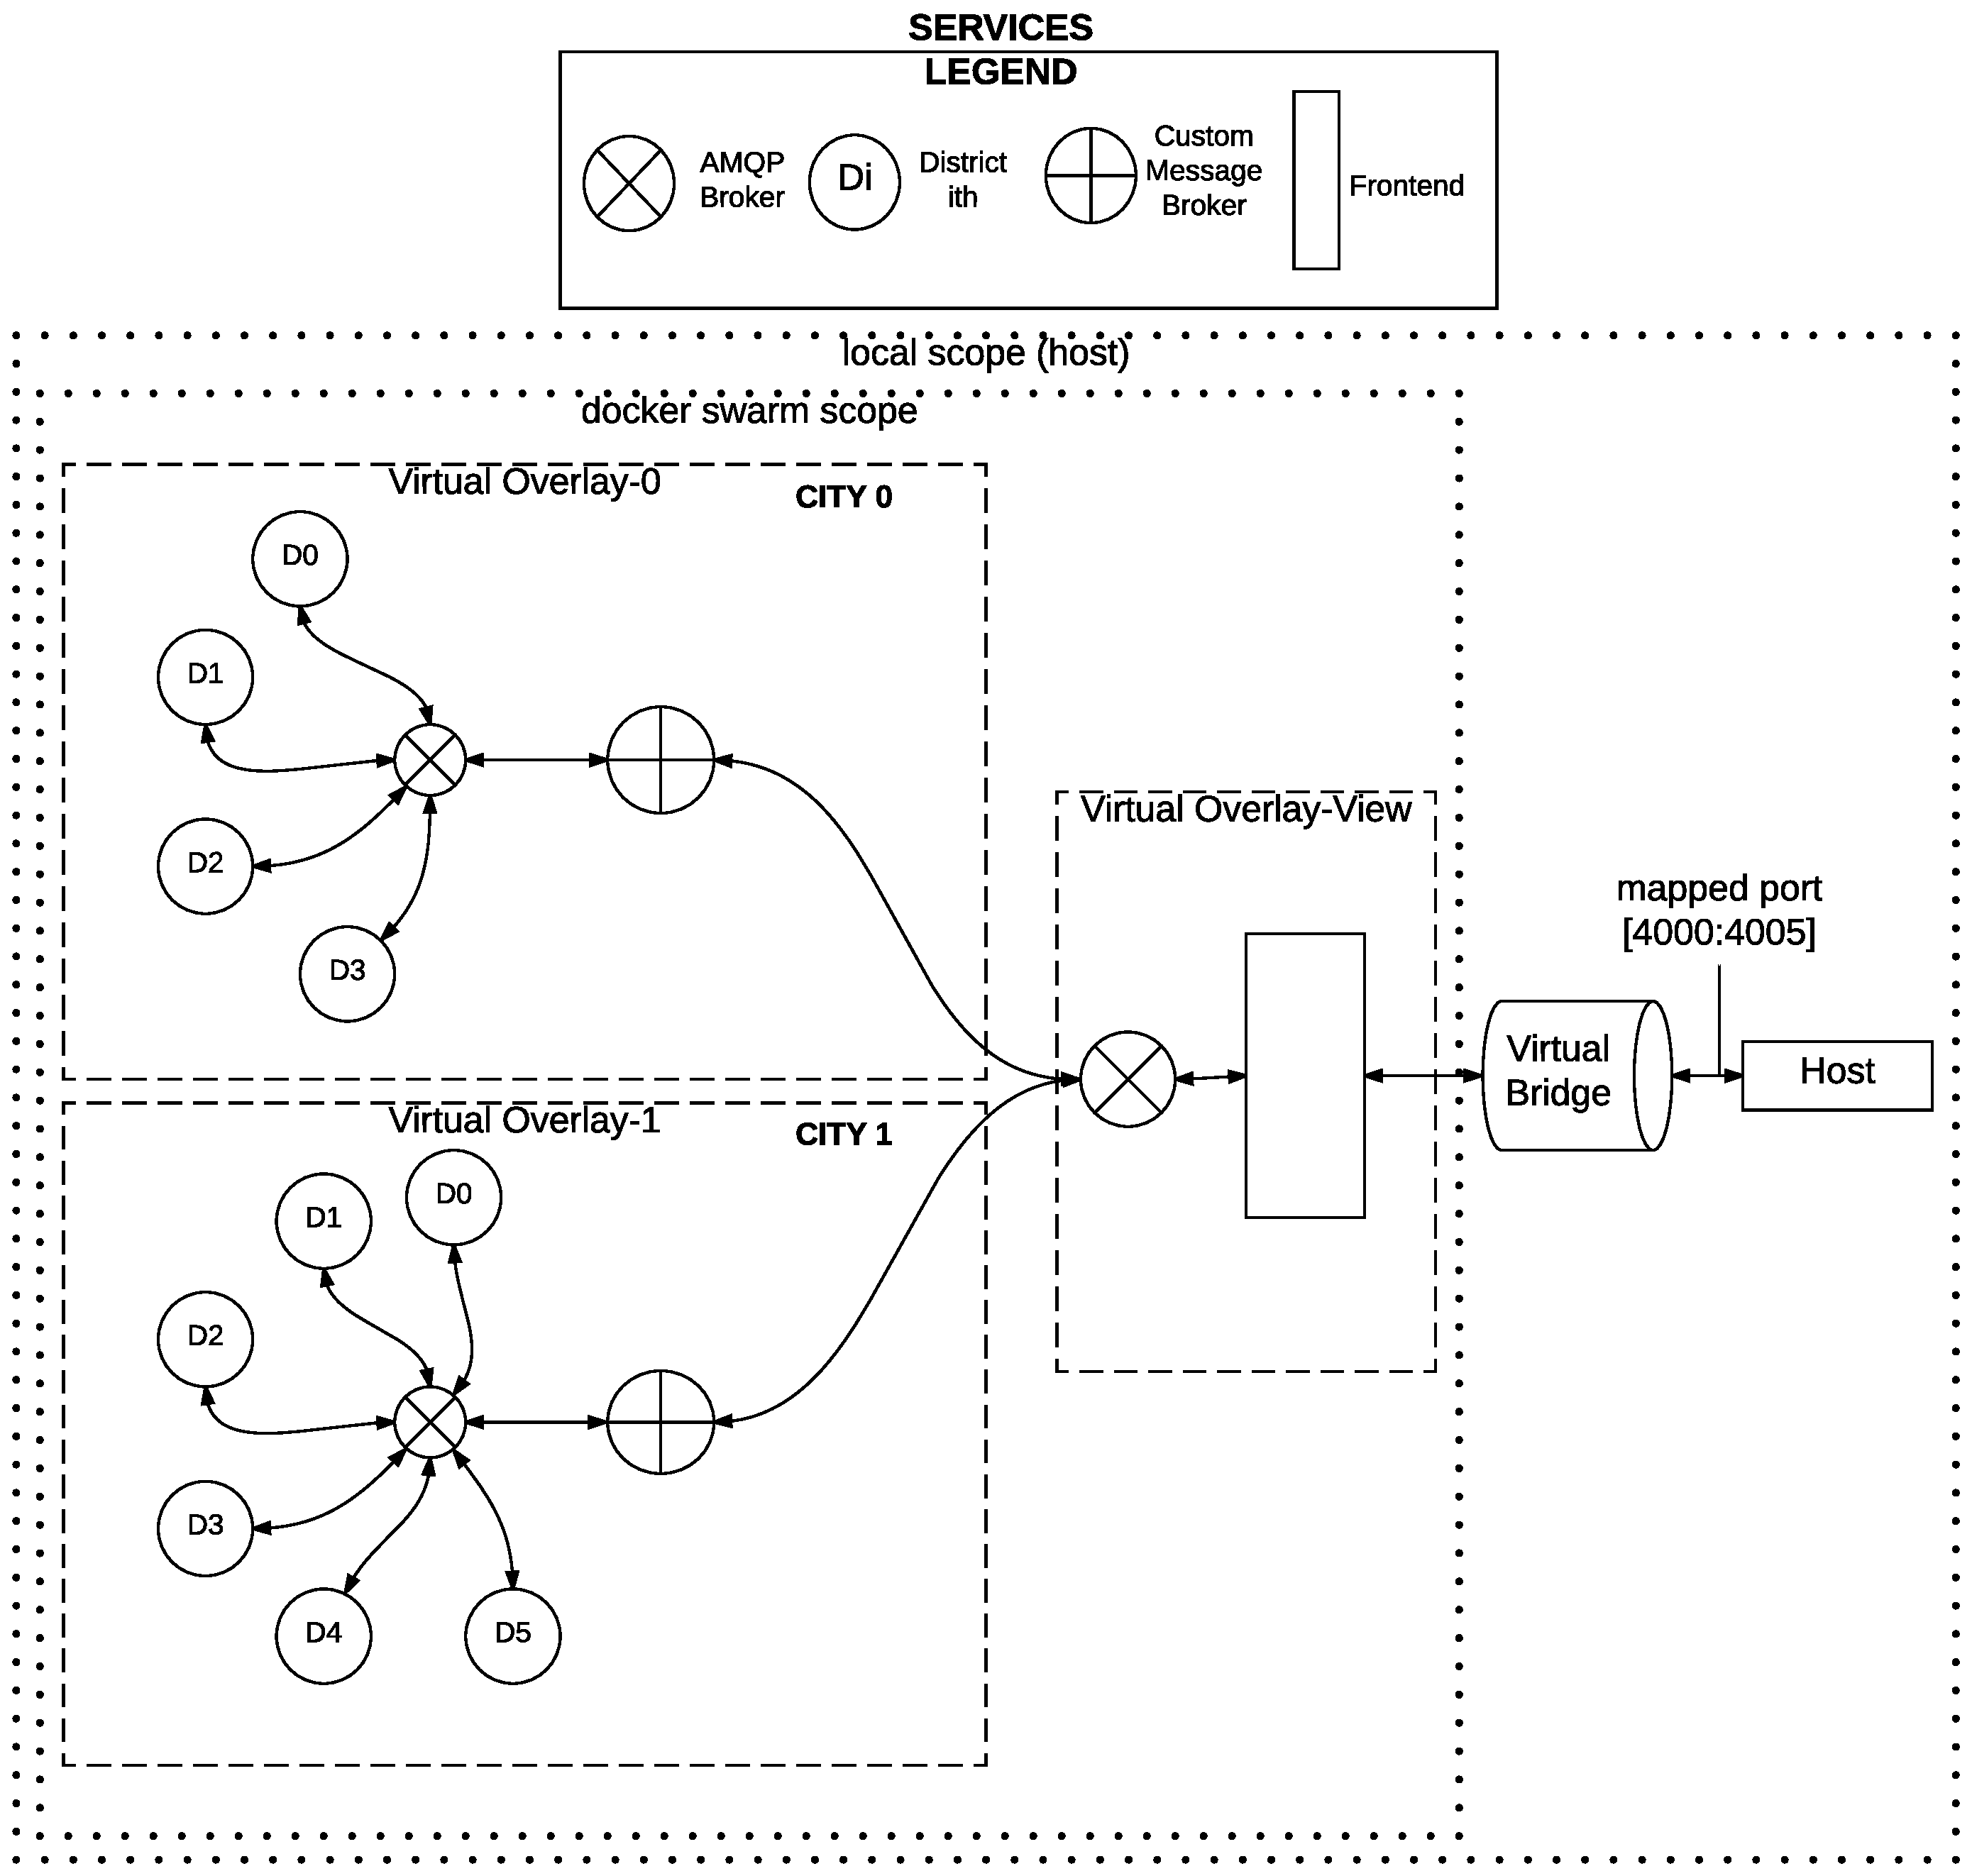
\includegraphics[scale=0.5,keepaspectratio]{images/user-man/app/deploy.eps}
\caption{Example of the deployed system}
\label{fig:deploy-sys}
\end{figure}